\subsection{FL Architectures}

FL comes in two broad structural categories.
Cross-silo or enterprise FL gets used in large data centers or multinational companies.
Each learner represents a single institution or participating group.
There are only around ten to a few dozen learners involved.
Cross-silo FL considers the identity of the parties for training and verification.
Generally, every individual local update from every learner at every training round is significant.
Fallouts and failures of individual learners are serious.
Cross-device FL can include hundreds or millions of devices, primarily edge/IoT devices.
Due to this great pool of learners, only a subset typically trains per round.
The identities of the participating learners are usually unimportant.
Due to the nature of these devices and their environments, cross-device FL needs to manage special challenges.
Challenges include non-IID data, heterogeneous device hardware, different network conditions, learner outages, or stragglers.
Various techniques exist to navigate these challenging conditions, including specialized algorithms for aggregation or learner selection.
These strategies can consider bias, availability, resources, and battery life.
\vspace{2mm}
\newline\textbf{From now on, when we mention FL in this work, we mean cross-device FL because FLOps focuses on cross-device workloads.}
\vspace{5mm}
\newline
Different FL architectures exist to support large-scale FL environments.
FLOps wants to benefit from the unique three-tiered Oakestra \cite{paper:oakestra_usenix} architecture.
Such a scenario has two main challenges.
The first challenge is managing a massive number of connections and aggregations.
The second one is reducing the negative impact of straggling learner updates.
The problem with using a single aggregator, as seen in \ref{fig:basic_fl_intro}, is that this single aggregator becomes a communication bottleneck.
Additionally, per-round training latency is limited by the slowest participating learner.
Thus, stragglers turn into another bottleneck.
The following is an overview of prominent FL architectures.

\subsubsection{Clustered FL}

\begin{figure}[b]
    \centering
    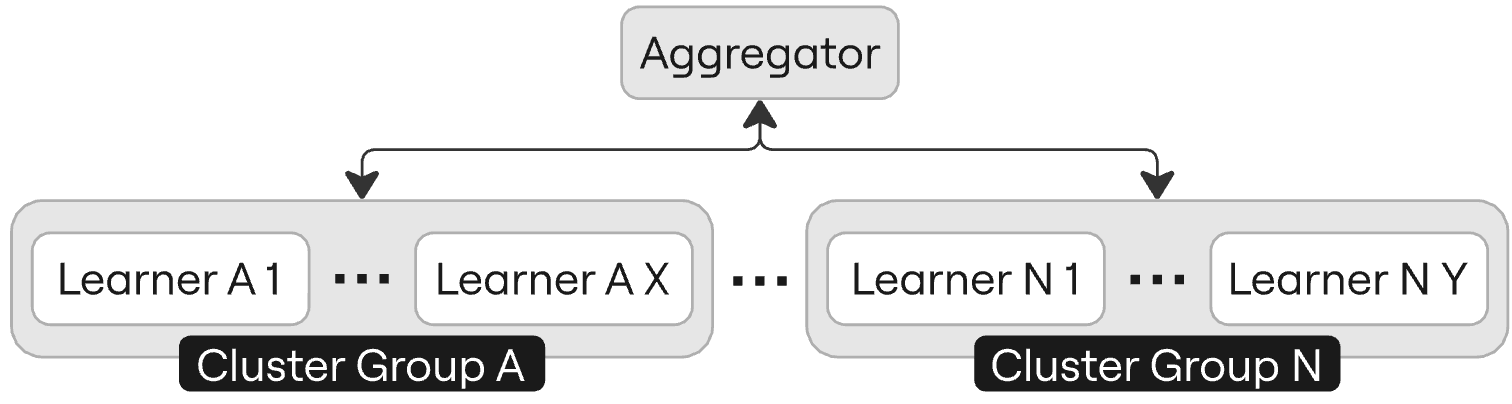
\includegraphics[width=\textwidth]{clustered_fl.png}
    \caption{Clustered FL Architecture}
    \label{fig:clustered_fl}
\end{figure}
Figure \ref{fig:clustered_fl} shows the Clustered FL (CFL) architecture that groups similar learners into clusters.
CFL can form clusters based on local data distribution, training latency, available hardware, or geographical location.
The issue of the singular aggregator as a bottleneck persists.
The main challenge for CFL is choosing a suitable clustering strategy and criteria for the concrete use case.
If the criteria are biased, updates from preferred clusters might be heavily favored, resulting in a biased global model with bad generalization.
Another task is to properly profile the nodes to match them to the correct cluster.
The entire cluster suffers if a slow outlier is present in a cluster.
Node properties can vary over time, so cluster membership has to be dynamic.
Too intrusive profiling can lead to compromised privacy.
The benefits of CFL are its ease of implementation, familiar architecture to classic FL, and flexibility to tune clustering/selection dynamically.
CFL can be combined with other architectures.
A downside of CFL is that a proper clustering strategy is use-case-dependent and challenging to optimize.
CFL does not really solve scalability issues on its own.
Its clustering overhead becomes critical with larger numbers of nodes.
\cite{
    paper:cluster_based_secure_aggregation_for_fl,
    paper:fedat_high_performance_communication_efficient_fl_with_asynch_tiers,
    book:fl,paper:decentralized_edge_intelligence_dynamic_resource_allocation_framework_hfl}

\subsubsection{Hierarchical FL}
\begin{figure}[b]
    \centering
    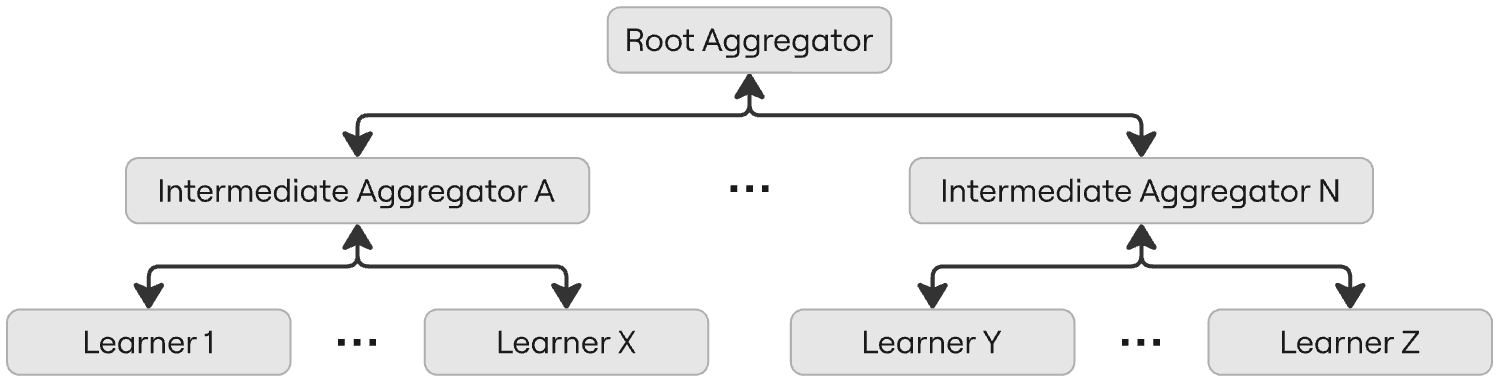
\includegraphics[width=\textwidth]{hfl_architecture.png}
    \caption{Hierarchical FL Architecture}
    \label{fig:hfl_architecture}
\end{figure}
Figure \ref{fig:hfl_architecture} depicts the hierarchical FL (HFL) architecture.
In HFL, the root aggregator delegates and distributes the aggregation task to intermediate aggregators.
HFL can have multiple layers of intermediate aggregators.
Each intermediate aggregator and its connected learners resemble an instance of classic FL.
After aggregating an intermediate model, the intermediate aggregators send their parameters upstream to the root aggregator.
The root combines the intermediate parameters into global ones and sends them downstream for further FL rounds.
HFL's structure requires changing the underlying FL architecture.

The proper design and implementation, and the assignment of learners to aggregators determine the success of one's FL setup.
For example, if too many learners are attached to a given aggregator, that aggregator becomes a bottleneck.
The intermediate aggregated model can be biased if too few learners are assigned.
Thus, the infrastructure resources and management costs become unjustified for the small number of learners.
A management overhead arises with more components, including handling fault tolerance, monitoring, synchronizing, and balancing.
Bad synchronization can amplify straggler problems.
Balancing refers to combining and harmonizing intermediate parameters to get a good global model.
These findings show that special FL architectures, such as HFL, require careful consideration and correct implementation.
\cite{book:fl,paper:decentralized_edge_intelligence_dynamic_resource_allocation_framework_hfl,hpfl_over_massive_mobile_edge_computing_networks}

The benefits of HFL are its dynamic scalability and load balancing.
One can easily add or remove intermediate aggregators and their connected learners.
Due to this distribution of load and aggregation, each aggregator, including the root, is less likely to face bottleneck issues.
One can combine HFL with CFL, where each intermediate aggregator is responsible for one or multiple clusters.
The downsides of HFL are communication and management overheads.
More components lead to more transmitted messages.
These messages all need to be secured and encrypted.
With more components and nodes, adversaries can take advantage of more possible backdoors.
HFL provides a powerful way to improve scalability for FL if done right.
\cite{
    paper:deploying_fl_in_hierarchical_edge_architecture,
    paper:hfl_with_momentum_acceleration_in_multi_tier_networks,
    paper:hfl_with_privacy,
    paper:decentralized_edge_intelligence_dynamic_resource_allocation_framework_hfl,
    book:fl,
    hpfl_over_massive_mobile_edge_computing_networks}


\subsubsection{Decentralized FL}
Decentralized FL does not require a central aggregator.
Instead, it operates on a peer-to-peer basis via a blockchain.
That way, the centralized communication bottleneck gets resolved.
The blockchain represents the global model.
Learners train in parallel.
Each locally trained update gets a version.
Based on this version, random clients are chosen for aggregation.
The results get appended to the blockchain, and the model version is incremented. \cite{book:fl}

\subsubsection{Asynchronous FL}
Asynchronous FL allows learners to train continuously and freely push their updates to the aggregator.
This method eliminates stragglers and dropout problems because a training round does not need to wait or handle outliers and timeouts.
A new issue of staleness arises when updates are merged into the global model that took a very long time to complete.
Such an update used a now outdated version of the global model.
As a result, the global model is partially reverted to an older state.
Asynchronous FL can be combined with other architectures. \cite{book:fl}